% Options for packages loaded elsewhere
\PassOptionsToPackage{unicode}{hyperref}
\PassOptionsToPackage{hyphens}{url}
%
\documentclass[
]{article}
\usepackage{amsmath,amssymb}
\usepackage{iftex}
\ifPDFTeX
  \usepackage[T1]{fontenc}
  \usepackage[utf8]{inputenc}
  \usepackage{textcomp} % provide euro and other symbols
\else % if luatex or xetex
  \usepackage{unicode-math} % this also loads fontspec
  \defaultfontfeatures{Scale=MatchLowercase}
  \defaultfontfeatures[\rmfamily]{Ligatures=TeX,Scale=1}
\fi
\usepackage{lmodern}
\ifPDFTeX\else
  % xetex/luatex font selection
\fi
% Use upquote if available, for straight quotes in verbatim environments
\IfFileExists{upquote.sty}{\usepackage{upquote}}{}
\IfFileExists{microtype.sty}{% use microtype if available
  \usepackage[]{microtype}
  \UseMicrotypeSet[protrusion]{basicmath} % disable protrusion for tt fonts
}{}
\makeatletter
\@ifundefined{KOMAClassName}{% if non-KOMA class
  \IfFileExists{parskip.sty}{%
    \usepackage{parskip}
  }{% else
    \setlength{\parindent}{0pt}
    \setlength{\parskip}{6pt plus 2pt minus 1pt}}
}{% if KOMA class
  \KOMAoptions{parskip=half}}
\makeatother
\usepackage{xcolor}
\usepackage[margin=1in]{geometry}
\usepackage{graphicx}
\makeatletter
\def\maxwidth{\ifdim\Gin@nat@width>\linewidth\linewidth\else\Gin@nat@width\fi}
\def\maxheight{\ifdim\Gin@nat@height>\textheight\textheight\else\Gin@nat@height\fi}
\makeatother
% Scale images if necessary, so that they will not overflow the page
% margins by default, and it is still possible to overwrite the defaults
% using explicit options in \includegraphics[width, height, ...]{}
\setkeys{Gin}{width=\maxwidth,height=\maxheight,keepaspectratio}
% Set default figure placement to htbp
\makeatletter
\def\fps@figure{htbp}
\makeatother
\setlength{\emergencystretch}{3em} % prevent overfull lines
\providecommand{\tightlist}{%
  \setlength{\itemsep}{0pt}\setlength{\parskip}{0pt}}
\setcounter{secnumdepth}{-\maxdimen} % remove section numbering
\usepackage{multicol}
\usepackage{natbib}
\usepackage{graphicx}
\usepackage{caption}
\ifLuaTeX
  \usepackage{selnolig}  % disable illegal ligatures
\fi
\usepackage{bookmark}
\IfFileExists{xurl.sty}{\usepackage{xurl}}{} % add URL line breaks if available
\urlstyle{same}
\hypersetup{
  pdftitle={Linux Authentication and PAM},
  pdfauthor={Henry Roeth},
  hidelinks,
  pdfcreator={LaTeX via pandoc}}

\title{Linux Authentication and PAM}
\usepackage{etoolbox}
\makeatletter
\providecommand{\subtitle}[1]{% add subtitle to \maketitle
  \apptocmd{\@title}{\par {\large #1 \par}}{}{}
}
\makeatother
\subtitle{Face Recognition}
\author{Henry Roeth}
\date{2024-02-16}

\begin{document}
\maketitle
\begin{abstract}
In computer security, authentication is the process of confirming
someone is who they claim to be when attempting to access any kind of
computer system through the confirmation of something they have,
something they know, or something they are. It is important to always
maintain and improve the integrity of computer systems' authentication
schemes as new security threats arise. The Linux kernel invokes the
standard Unix authentication process across the majority of its
applications. However, as new forms of authentication are developed, it
is inefficient to individually reconfigure applications such that the
desired authentication scheme is incorporated. The PAM (Pluggable
Authentication Module) mechanism in Linux integrates various low-level
authentication schemes into a high-level API, allowing programs that
require some form of authentication to be developed independently from
the desired authentication scheme. This integrated research aims to
demonstrate the function and importance of PAM in Linux authentication
with the invocation of a face recognition PAM security module. Real-time
face detection and recognition is performed using the Haar Cascade
Classifier and the LBPH (Local Binary Patterns Histograms) feature-based
face recognition method.
\end{abstract}

\begin{multicols}{2}

\section{Introduction}
The Linux kernel invokes the standard Unix authentication process across most of its applications (e.g., common-auth, sshd, su, and sudo). When developers are creating and updating applications, it would prove quite inefficient to individually reconfigure application logic such that it aligns with the newly desired authentication scheme. This would mean restructuring code and requiring other dependencies. With this in mind, developers need a way to invoke authentication schemes independently from applications, allowing for a more modular approach. This enables programs to run separately. Much like it's father kernel (Unix) the Linux kernel invokes these modular authentication schemes via the PAM (Pluggable Authentication Module) mechanism. One might think of this as a multitool. Just as a multitool can have different tools for various purposes like cutting, screwing, or opening, PAM provides different authentication methods for Linux. Depending on what you need to authenticate—be it through passwords, biometrics, or other means—you can plug in the appropriate tool/module into PAM to handle the authentication process effectively. This integrated research aims to display this function with the creation of a modular authentication scheme—face recognition.

\section{Overview of Linux Authentication}
Linux authentication involves several components. Centrally are the /etc/passwd and /etc/shadow files. In `/etc/passwd`, user account information such as usernames, user IDs, group IDs, and home directories are stored. The tangible passwords are more securely stored in `/etc/shadow`. It is here where there are hashed passwords and other security-related information. Each line in `/etc/shadow` represents a user account and includes uniquely populated fields like usernames, encrypted passwords, password aging and expiration details, and account lockout information. When any user attempts to login to the machine, the system hashes the entered password using the same algorithm as the one stored in /etc/shadow. If the hashed passwords match, access is granted to the user. More specifically, hashing involves the conversion of a password into a fixed-length string of characters using a cryptographic hash function. This process is irreversible, meaning the original password cannot be easily derived from the hash. Another additional measure of security that is implemented in the hashing process is salting. Salting is where a random value (a salt) is added to the password before hashing. This prevents attackers from using precomputed hash tables, also known as rainbow tables, to crack passwords. These unique fields in the /etc/shadow file are separated by colons, with each field serving a specific purpose. These fields may typically include the username, the hashed password, the last password date, the minimum and maximum password age, the password warning period, the password inactivity period, the account expiration date, and the account expiration date warning. To summarize, the integrity of the Linux authentication process relies on secure data storage of hashed passwords, salting for additional security, and an automated management system of user account information. As this relates to PAM, the invoked module (found in the directory /lib/*/security) is the primary logic to which the input password is hashed and compared to the corresponding hash in the /etc/shadow file; it is then followed by either a success or failure being return to the PAM mechanism.

\section{Hashing}
Hashing plays a pivotal role in Linux authentication mechanisms, safeguarding user credentials stored on the system. In Linux, password hashes are typically generated using cryptographic hash functions such as SHA-256 or SHA-512. When a user sets or updates their password, the system computes the hash of the password and stores it in the system's password file (`/etc/shadow`). When a user attempts to log in, the system hashes the provided password using the same algorithm and compares it with the stored hash in the password file. If the hashes match, access is granted. Otherwise, access is denied. This process ensures that even if an attacker gains access to the password file, obtaining the original passwords is exceedingly difficult due to the one-way nature of cryptographic hashing. According to \cite{doe2020survey}, hash functions are crucial for data integrity verification in authentication systems, emphasizing properties like collision resistance, which are essential for robust security implementations.

\section{Salts}
Salts are key in enhancing the security of password storage in Linux. When a user sets or changes their password, a random salt is generated and combined with the password before hashing. This salt is then stored alongside the hashed password in the system's password file. The purpose of the salt is to prevent attackers from using precomputed hash tables, such as rainbow tables, to quickly determine the original password from its hash. By adding a unique salt to each password before hashing, even if two users have the same password, their hashed values will be different due to the different salts used. Consequently, rainbow table attacks become impractical, as attackers would need to generate a new table for each unique salt value. This significantly increases the complexity and time required for password cracking attempts. Salting effectively mitigates various password-based attacks, thereby strengthening the overall security of the Linux authentication system (\cite{smith2021importance}).

\end{multicols}

\begin{figure}[htbp]
  \centering
  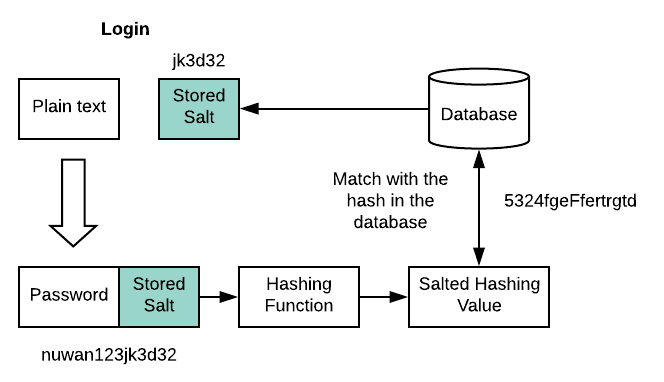
\includegraphics[width=0.4\linewidth]{images/salting.png}
  \caption{Linux Salting Process}
\end{figure}

\begin{multicols}{2}

\section{PAM Configuration}
Pluggable Authentication Modules (PAM) constitute a critical component of Linux systems, providing a flexible framework for authentication management. PAM enables system administrators to configure authentication policies independently of the applications requiring authentication, thus promoting modularity and security. Central to PAM's functionality are its configuration files located in `/etc/pam.d/`, which define the authentication rules for specific services or applications. These configuration files specify the modules to be invoked during authentication, such as password verification, account validation, and session management. Each module performs a specific authentication task, allowing administrators to tailor authentication mechanisms according to their security requirements. PAM modules can employ various authentication methods, including traditional password-based authentication, token-based authentication, biometric authentication, and multi-factor authentication. Additionally, PAM's modular design allows for the inclusion of custom authentication modules located in `/lib/*/security`, enabling further customization and integration with external authentication services, such as LDAP or Kerberos. This flexibility, coupled with PAM's extensibility, makes it a cornerstone of Linux security, facilitating robust authentication mechanisms that can adapt to diverse system architectures and security policies (\cite{jones2022importance}). 

\end{multicols}

\begin{figure}[htbp]
  \centering
  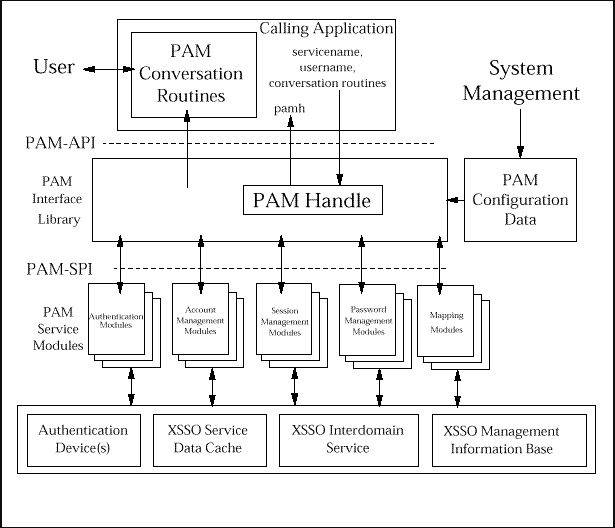
\includegraphics[width=0.4\linewidth]{images/pam_configuration.png}
  \caption{PAM System Framework}
\end{figure}

\begin{multicols}{2}

\section{Biometrics}
Biometrics, a field at the intersection of computer science and biology, offers innovative solutions for identity verification and access control. It involves the measurement and analysis of unique physical or behavioral characteristics to establish an individual's identity. Unlike traditional authentication methods like passwords or tokens, which can be lost, stolen, or forgotten, biometric traits are inherently linked to a person and are difficult to replicate. Biometric systems typically capture data from various sources, including fingerprints, iris patterns, facial features, voice patterns, and even behavioral traits like gait or typing patterns. These biometric data are then processed and converted into mathematical representations, often referred to as templates or biometric signatures. During authentication, a user's biometric data is captured and compared against the stored template in a database. If the biometric features match within an acceptable threshold, access is granted. The use of biometrics offers several advantages, including increased security, convenience, and resistance to fraud. However, challenges such as privacy concerns, accuracy, and susceptibility to spoofing techniques remain significant areas of research and development in the field. Nonetheless, with advancements in technology and algorithms, biometrics continues to gain traction in various domains, including law enforcement, border control, banking, and mobile devices (\cite{wang2023introduction}).

\section{Machine Learning}

Machine learning, a subset of artificial intelligence, has revolutionized various fields by enabling systems to learn from data and make predictions or decisions without explicit programming. In the context of face recognition, machine learning algorithms play a pivotal role in extracting meaningful features from facial images and identifying patterns that distinguish one individual from another. These algorithms can be trained on vast datasets of labeled facial images, learning to recognize unique facial characteristics such as the arrangement of eyes, nose, and mouth, as well as more subtle cues like skin texture and facial expressions. Convolutional Neural Networks (CNNs) are particularly effective for face recognition tasks, leveraging hierarchical layers to automatically learn relevant features at different levels of abstraction. Additionally, techniques like transfer learning allow pre-trained models to be fine-tuned on specific face recognition tasks, enhancing performance even with limited training data. Despite the remarkable progress in face recognition enabled by machine learning, challenges such as robustness to variations in pose, illumination, and occlusion persist, driving ongoing research efforts to develop more accurate and reliable face recognition systems (\cite{schwarz2021machine}). Furthermore, within the realm of face recognition, one prominent method that leverages machine learning techniques is Local Binary Pattern Histograms (LBPH). LBPH is a texture-based approach that captures local patterns in an image and constructs histograms of these patterns to represent the image's texture. This method has gained popularity for its simplicity, computational efficiency, and effectiveness, particularly in scenarios with limited training data or computational resources. By incorporating machine learning principles, LBPH algorithms can adapt and learn discriminative patterns from facial images, contributing to the advancement of robust and accurate face recognition systems.

\section{Haar Cascade Classifier}
The Haar Cascade Classifier is a widely used object detection algorithm in computer vision, particularly in tasks such as face detection. Developed by Viola and Jones in 2001, this method utilizes a set of simple rectangular features called Haar-like features, which are extracted from image windows at different scales and positions. These features are then fed into a cascade of classifiers, each of which efficiently distinguishes between regions of an image that likely contain the object of interest and those that do not. The cascade structure allows for fast rejection of non-object regions, enabling real-time processing of images or video streams. While originally introduced for face detection, the Haar Cascade Classifier has since been applied to various object detection tasks, demonstrating its versatility and effectiveness in detecting objects in complex scenes (\cite{viola2004robust}).

\end{multicols}

\begin{figure}[htbp]
  \centering
  
\includegraphics[width=0.4\linewidth]{images/haar_features.png}
  \caption{Haar-Like Features}
\end{figure}

\begin{figure}[htbp]
  \centering
  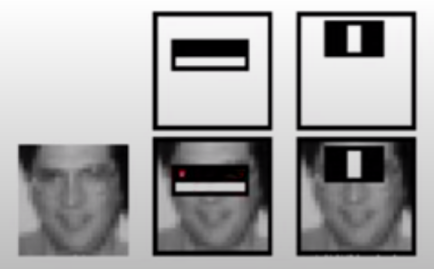
\includegraphics[width=0.4\linewidth]{images/haar_features_1.png}
  \caption{Application of Haar-Like Features}
\end{figure}

\begin{multicols}{2}

\section{Local Binary Pattern Historgrams}
Local Binary Patterns (LBPH) remains a stalwart in face recognition, esteemed for its robustness and adaptability to diverse conditions. This method dissects facial images into local neighborhoods, each representing a distinct region of interest. LBPH meticulously examines texture information encoded in pixel intensity values. Its process involves assessing the relationship between the central pixel and its surrounding neighbors, encapsulated within a circular neighborhood. Herein lies LBPH's efficacy: binary encoding of this relationship. For each pixel, LBPH determines whether its intensity surpasses or falls short of its neighbors'. Pixels with higher intensities receive a binary value of 1; otherwise, they receive 0. This binary representation, akin to a digital fingerprint, captures intricate texture details intrinsic to the facial region. By traversing the entire image and repeating this process for every pixel, LBPH assembles a comprehensive mosaic of texture patterns, each encoded into a binary string. These strings, emblematic of the texture variations within each neighborhood, are transformed into decimal values. LBPH distills these values into histograms, encapsulating texture within each neighborhood. Subsequently, these histograms, like miniature texture portraits, are concatenated into a feature vector, representing that of the entire facial image. LBPH transcends limitations of traditional face recognition techniques, surmounting challenges posed by illumination variations, pose changes, and facial expressions (\cite{ahonen2004}; \cite{tan2007}). Thus, LBPH emerges as an efficient method in face recognition, indispensable in applications from security systems to human-computer interaction interfaces.

\end{multicols}

\begin{figure}[htbp]
  \centering
  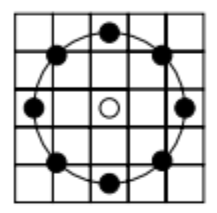
\includegraphics[width=0.4\linewidth]{images/lbph.png}
  \caption{Local Binary Pattern}
\end{figure}

\begin{figure}[htbp]
  \centering
  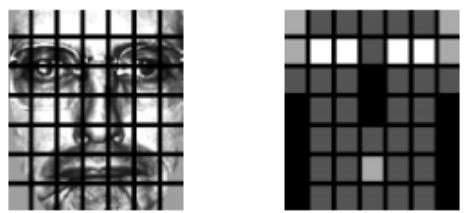
\includegraphics[width=0.4\linewidth]{images/lbph_1.png}
  \caption{LBP Application}
\end{figure}

\begin{figure}[htbp]
  \centering
  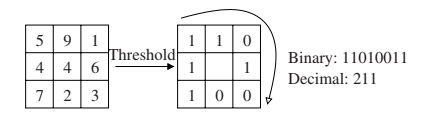
\includegraphics[width=0.4\linewidth]{images/lbph_2.png}
  \caption{Decimal Value Calculation Process}
\end{figure}

\begin{multicols}{2}

\section{PAM Configuraiton Files}
PAM configuration files serve as the cornerstone of user authentication in Linux systems, orchestrating a seamless interaction between applications and authentication mechanisms. At the crux of PAM configuration files lie policy lines, delineating the authentication process for specific applications in great detail. Each policy line comprises several fields, meticulously crafted to orchestrate a tailored authentication workflow. The first field, the module type, specifies the category of authentication module to be invoked, ranging from account and session management to the actual authentication logic. Following this, the control flag dictates the behavior of the module, controlling aspects such as whether authentication is required to proceed (required), whether failure should halt the authentication process (requisite), or whether the success of one module should automatically grant access (sufficient). Subsequently, the module path denotes the location of the authentication module's executable file, facilitating its invocation during the authentication process. Parameters, the next field, enable fine-grained customization of module behavior, allowing administrators to specify additional options or configurations. Each parameter is passed to the module upon invocation, influencing its execution and outcome. Through judicious arrangement and configuration of these policy lines, administrators can tailor authentication workflows to meet the security requirements of individual applications, ensuring a fine balance between security and usability. When an application requests authentication, PAM dynamically assembles the configured modules and executes them in the specified order, passing control from one module to the next in a stack-like structure. Each module performs a specific authentication task, such as verifying passwords, checking user permissions, or enforcing multifactor authentication. By abstracting authentication from application logic, PAM enhances system security and simplifies management, facilitating centralized control over authentication policies across the entire system (\cite{stallings2020}; \cite{love2010}).

\end{multicols}

\begin{figure}[htbp]
  \centering
  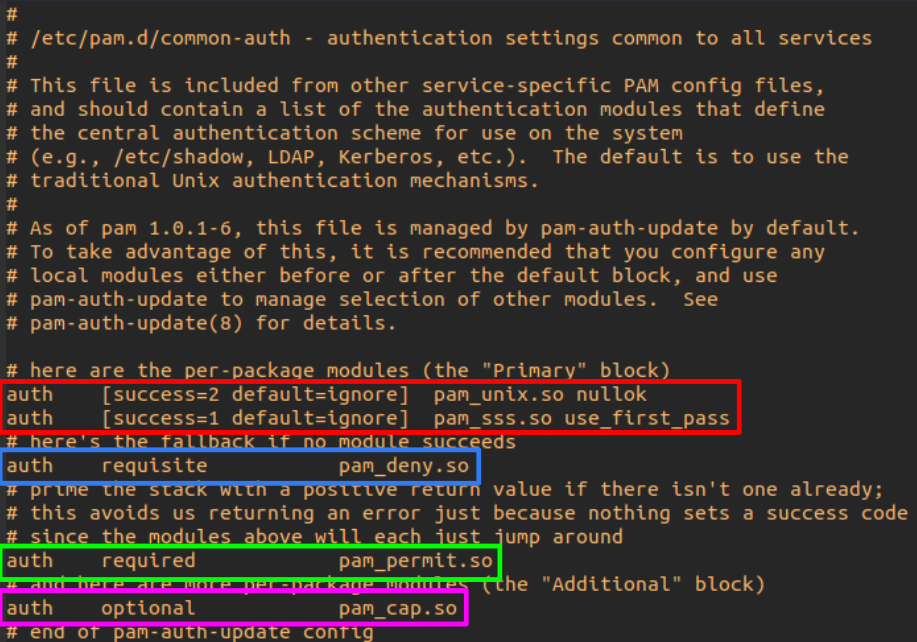
\includegraphics[width=0.4\linewidth]{images/common-auth.png}
  \caption{Module Invocation in `common-auth` PAM Configuration File}
\end{figure}

\bibliographystyle{apalike}
\bibliography{irc_1_ref.bib}

\end{document}
